
\section{Issues and Motivations}
\label{sec:motivations}

Causal broadcast is a communication primitive that allows a process to send
messages to all processes of its distributed system. Message deliveries follow
the happen before relationship. If the sending of a message $m$ precedes the
sending of a message $m'$ then all processes that deliver these two messages
need to deliver $m$ before $m'$. Otherwise they deliver them in any order. Each
process may receive a message multiple times but it delivers it exactly once.

Causal broadcast relies on reliable broadcast. First, it guarantees that all
correct processes eventually receive broadcast messages. Gossiping constitutes
an efficient mean to reliably disseminate messages to large systems. Each
process maintains a partial view considerably smaller than the whole system
membership. When a process broadcasts a message, it sends it to its partial
view; each process that receives such message forwards it to its partial
view. Broadcast messages reach all processes either directly or transitively.

\begin{figure*}
  \begin{center}
    \subfloat[Part A][\label{fig:generalpurgeA}Process~A broadcasts $a$. It expects 
    two copies of $a$.]
    {
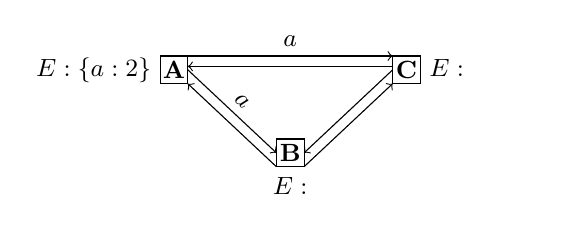
\begin{tikzpicture}[scale=1]
  
  \small
  
  \newcommand\X{210/5pt};
  \newcommand\Y{30pt};
  
  % \draw[->] ( -0.5*\X, 0.5*\Y) -- ( -5+0*\X, 0*\Y);
  % \draw[->] ( -0.5*\X, 0*\Y) -- ( -5+0*\X, 0*\Y);
  % \draw[->] ( -0.5*\X, -0.5*\Y) -- ( -5+0*\X, 0*\Y);  

  \draw[fill=white] (0*\X, 0*\Y) node{\textbf{A}} +(-5pt, -5pt) rectangle +(5pt, 5pt);
  \draw (-5+0*\X, 0*\Y) node[left]{$E: \{a:2\}$};
  \draw[fill=white] (1*\X, -1*\Y) node{\textbf{B}} +(-5pt, -5pt) rectangle +(5pt, 5pt);
  \draw (1*\X, -5-1*\Y) node[below]{$E: \varnothing$\vphantom{$\{$}};
  \draw[fill=white] (2*\X,  0*\Y) node{\textbf{C}} +(-5pt, -5pt) rectangle +(5pt, 5pt);
  \draw (5+2*\X, 0*\Y) node[right]{$E: \varnothing$\vphantom{$\{$}};
  \draw (5+2*\X, 0*\Y) node[right]{\phantom{$E: \{a:1\}$}};

  \draw[->](5+0*\X, 0*\Y) -- node[sloped, above]{$a$} (-5+1*\X, -1*\Y); %% A->B
  \draw[<-](5+0*\X, -5+0*\Y) -- (-5+1*\X, -5-1*\Y); %% A<-B

  \draw[->](5+0*\X, 5+0*\Y) -- node[above]{$a$} (-5+2*\X, 5+0*\Y); % A->C
  \draw[<-](5+0*\X,  1.25+ 0*\Y) -- (-5+2*\X,  1.25+ 0*\Y); % A<-C
 
  \draw[<-](5+1*\X, -1*\Y) -- (-5+2*\X, 0*\Y); %% B<-C
  \draw[->](5+1*\X, -5-1*\Y) -- (-5+2*\X, -5+0*\Y); %% B->C

  % \draw[->](5+2*\X, 0*\Y) -- ( 2.5*\X, 0*\Y);
\end{tikzpicture}}
    \hspace{10pt}
    \subfloat[Part B][\label{fig:generalpurgeB}Process~B and Process~C receive $a$. 
    They both expect another copy of $a$.]
    {
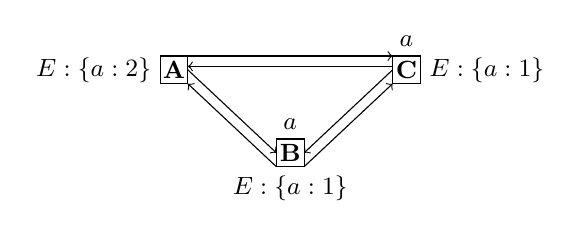
\begin{tikzpicture}[scale=1]
  
  \small
  
  \newcommand\X{210/5pt};
  \newcommand\Y{30pt};
  
  % \draw[->] ( -0.5*\X, 0.5*\Y) -- ( -5+0*\X, 0*\Y);
  % \draw[->] ( -0.5*\X, 0*\Y) -- ( -5+0*\X, 0*\Y);
  % \draw[->] ( -0.5*\X, -0.5*\Y) -- ( -5+0*\X, 0*\Y);  

  \draw[fill=white] (0*\X, 0*\Y) node{\textbf{A}} +(-5pt, -5pt) rectangle +(5pt, 5pt);
  \draw (-5+0*\X, 0*\Y) node[left]{$E: \{a:2\}$};
  \draw[fill=white] (1*\X, -1*\Y) node{\textbf{B}} +(-5pt, -5pt) rectangle +(5pt, 5pt);
  \draw (1*\X, 5-1*\Y) node[above]{$a$};
  \draw (1*\X, -5-1*\Y) node[below]{$E:\{a:1\}$};
  \draw[fill=white] (2*\X,  0*\Y) node{\textbf{C}} +(-5pt, -5pt) rectangle +(5pt, 5pt);
  \draw (2*\X, 5-0*\Y) node[above]{$a$};
  \draw (5+2*\X, 0*\Y) node[right]{$E:\{a:1\}$};

  \draw[->](5+0*\X, 0*\Y) -- (-5+1*\X, -1*\Y); %% A->B
  \draw[<-](5+0*\X, -5+0*\Y) -- (-5+1*\X, -5-1*\Y); %% A<-B

  \draw[->](5+0*\X, 5+0*\Y) -- (-5+2*\X, 5+0*\Y); % A->C
  \draw[<-](5+0*\X,  1.25+ 0*\Y) -- (-5+2*\X,  1.25+ 0*\Y); % A<-C
 
  \draw[<-](5+1*\X, -1*\Y) -- (-5+2*\X, 0*\Y); %% B<-C
  \draw[->](5+1*\X, -5-1*\Y) -- (-5+2*\X, -5+0*\Y); %% B->C

  % \draw[->](5+2*\X, 0*\Y) -- ( 2.5*\X, 0*\Y);
\end{tikzpicture}}
    \hspace{10pt}
    \subfloat[Part C][\label{fig:generalpurgeC}Process~B and Process~C forward $a$ 
    to their neighbors in a gossip fashion.]
    {
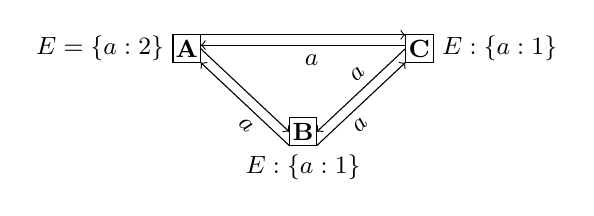
\begin{tikzpicture}[scale=1]
  
  \small
  
  \newcommand\X{210/5pt};
  \newcommand\Y{30pt};
  
  \draw[fill=white] (0*\X, 0*\Y) node{\textbf{A}} +(-5pt, -5pt) rectangle +(5pt, 5pt);
  \draw (-5+0*\X, 0*\Y) node[left]{$E = \{a:2\}$};
  \draw[fill=white] (1*\X, -1*\Y) node{\textbf{B}} +(-5pt, -5pt) rectangle +(5pt, 5pt);
%  \draw (1*\X, 5-1*\Y) node[above]{$a$};
  \draw (1*\X, -5-1*\Y) node[below]{$E:\{a:1\}$};
  \draw[fill=white] (2*\X,  0*\Y) node{\textbf{C}} +(-5pt, -5pt) rectangle +(5pt, 5pt);
%  \draw (2*\X, 5-0*\Y) node[above]{$a$};
  \draw (5+2*\X, 0*\Y) node[right]{$E:\{a:1\}$};

  \draw[->](5+0*\X, 0*\Y) -- (-5+1*\X, -1*\Y); %% A->B
  \draw[<-](5+0*\X, -5+0*\Y) -- node[sloped, below]{$\,\,\,\,\,\,\,a$} (-5+1*\X, -5-1*\Y); %% A<-B

  \draw[->](5+0*\X, 5+0*\Y) -- (-5+2*\X, 5+0*\Y); % A->C
  \draw[<-](5+0*\X,  1.25+ 0*\Y) -- node[below]{$\,\,\,\,a$} (-5+2*\X,  1.25+ 0*\Y); % A<-C
 
  \draw[<-](5+1*\X, -1*\Y) -- node[sloped,above]{$\,\,\,\,a$} (-5+2*\X, 0*\Y); %% B<-C
  \draw[->](5+1*\X, -5-1*\Y) -- node[sloped,below]{$a\,\,\,\,\,\,\,$}(-5+2*\X, -5+0*\Y); %% B->C

  % \draw[->](5+2*\X, 0*\Y) -- ( 2.5*\X, 0*\Y);
\end{tikzpicture}}
    \hspace{10pt}
    \subfloat[Part D][\label{fig:generalpurgeD}Process~B and Process~C forward $a$ 
    to their neighbors in a gossip fashion.]
    {
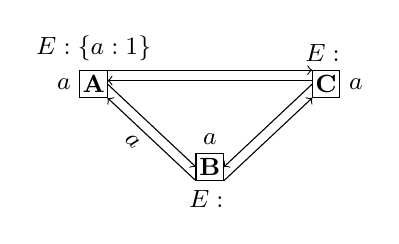
\begin{tikzpicture}[scale=1]
  
  \small
  
  \newcommand\X{210/5pt};
  \newcommand\Y{30pt};
  
  \draw[fill=white] (0*\X, 0*\Y) node{\textbf{A}} +(-5pt, -5pt) rectangle +(5pt, 5pt);
  \draw (-5+0*\X, 0*\Y) node[left]{$a$};
  \draw (0*\X, 5+0*\Y) node[above]{$E: \{a:\bm{1}\}$};
  \draw[fill=white] (1*\X, -1*\Y) node{\textbf{B}} +(-5pt, -5pt) rectangle +(5pt, 5pt);
  \draw (1*\X, 5-1*\Y) node[above]{$a$};
  \draw (1*\X, -5-1*\Y) node[below]{$E:\bm{\varnothing}$};%\vphantom{$\{$}};
  \draw[fill=white] (2*\X,  0*\Y) node{\textbf{C}} +(-5pt, -5pt) rectangle +(5pt, 5pt);
  \draw (5+2*\X, 0*\Y) node[right]{$a$};
  \draw (2*\X, 5+0*\Y) node[above]{$E:\bm{\varnothing}$};%\vphantom{$\{$}};
%  \draw (5+2*\X, 0*\Y) node[right]{\phantom{$E:\{a:1\}$}};

  \draw[->](5+0*\X, 0*\Y) -- (-5+1*\X, -1*\Y); %% A->B
  \draw[<-](5+0*\X, -5+0*\Y) -- node[sloped, below]{$a\,\,\,\,\,\,$} (-5+1*\X, -5-1*\Y); %% A<-B

  \draw[->](5+0*\X, 5+0*\Y) -- (-5+2*\X, 5+0*\Y); % A->C
  \draw[<-](5+0*\X,  1.25+ 0*\Y) -- (-5+2*\X,  1.25+ 0*\Y); % A<-C
 
  \draw[<-](5+1*\X, -1*\Y) -- (-5+2*\X, 0*\Y); %% B<-C
  \draw[->](5+1*\X, -5-1*\Y) -- (-5+2*\X, -5+0*\Y); %% B->C

  % \draw[->](5+2*\X, 0*\Y) -- ( 2.5*\X, 0*\Y);
\end{tikzpicture}}
    \hspace{10pt}
    \subfloat[Part E][\label{fig:generalpurgeE}Process~B and Process~C forward $a$ 
    to their neighbors in a gossip fashion.]
    {
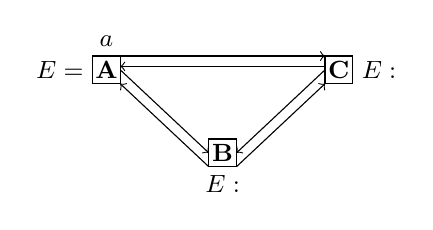
\begin{tikzpicture}[scale=1]
  
  \small
  
  \newcommand\X{210/5pt};
  \newcommand\Y{30pt};
  
  \draw[fill=white] (0*\X, 0*\Y) node{\textbf{A}} +(-5pt, -5pt) rectangle +(5pt, 5pt);
  \draw (0*\X, 5-0*\Y) node[above]{$a$};
  \draw (-5+0*\X, 0*\Y) node[left]{$E = \varnothing$};
  \draw[fill=white] (1*\X, -1*\Y) node{\textbf{B}} +(-5pt, -5pt) rectangle +(5pt, 5pt);
  \draw (1*\X, -5-1*\Y) node[below]{$E:\varnothing$};
  \draw[fill=white] (2*\X,  0*\Y) node{\textbf{C}} +(-5pt, -5pt) rectangle +(5pt, 5pt);
  \draw (5+2*\X, 0*\Y) node[right]{$E:\varnothing$};

  \draw[->](5+0*\X, 0*\Y) -- (-5+1*\X, -1*\Y); %% A->B
  \draw[<-](5+0*\X, -5+0*\Y) -- (-5+1*\X, -5-1*\Y); %% A<-B

  \draw[->](5+0*\X, 5+0*\Y) -- (-5+2*\X, 5+0*\Y); % A->C
  \draw[<-](5+0*\X,  1.25+ 0*\Y) -- (-5+2*\X,  1.25+ 0*\Y); % A<-C
 
  \draw[<-](5+1*\X, -1*\Y) -- (-5+2*\X, 0*\Y); %% B<-C
  \draw[->](5+1*\X, -5-1*\Y) -- (-5+2*\X, -5+0*\Y); %% B->C

  % \draw[->](5+2*\X, 0*\Y) -- ( 2.5*\X, 0*\Y);
\end{tikzpicture}}

    \caption{meow.}
  \end{center}
\end{figure*}


Second, reliable broadcast guarantees that each process delivers each broadcast
message exactly once, in spite of multiple receipts that can occur. A
lightweight implementation consists in recording the number of copies expected
after the first receipt. When the expected number of copies falls to zero, the
message will never be received again. Reliable broadcast purges its local
structure from this element. \TODO{Figure.}

Unfortunately, such implementation does not handle dynamic systems where
processes can join, leave, or self-reconfigure their partial view at any
time. \TODO{Figure.} 

To solve this issue, state-of-the-art protocols maintain a local vector the size
of which increases linearly with the number of processes that ever broadcast a
message. They eventually become overcostly in dynamic settings.

In this paper, we exploit and extend \PCBROADCAST to provide a causal broadcast
middleware that is lightweight in terms of local memory consumption, and message
overhead. The next section describes the proposed protocol.

%%% Local Variables:
%%% mode: latex
%%% TeX-master: "../paper.tex"
%%% End:
